%%%%%%%% READ ME %%%%%%%%%%%%%%%%%
% COMPILE dropcluster_appendix.tex first

\documentclass{article}

% Recommended, but optional, packages for figures and better typesetting:
\usepackage{microtype}
\usepackage{graphicx}
\usepackage{subfigure}
\usepackage{booktabs} % for professional tables
\usepackage{multirow}

% hyperref makes hyperlinks in the resulting PDF.
% If your build breaks (sometimes temporarily if a hyperlink spans a page)
% please comment out the following usepackage line and replace
% \usepackage{icml2020} with \usepackage[nohyperref]{icml2020} above.
\usepackage{hyperref}
% \usepackage{cleveref}

% Attempt to make hyperref and algorithmic work together better:
\newcommand{\theHalgorithm}{\arabic{algorithm}}

% Use the following line for the initial blind version submitted for review:
\usepackage{icml2020}
% If accepted, instead use the following line for the camera-ready submission:
%\usepackage[accepted]{icml2020}

% OUR PACKAGES
\usepackage{amssymb}
\usepackage{amsbsy}
\usepackage{amsmath}
%\usepackage{breqn}
\def\bx{\mathbf{x}}
\def\bX{\mathbf{X}}
\def\bz{\mathbf{z}}
\def\bZ{\mathbf{Z}}
\usepackage{amsthm}
\newtheorem{thm}{Theorem}[section] % reset theorem numbering for each chapter
\theoremstyle{plain}
\newtheorem{assumption}{Assumption}[section]
\theoremstyle{definition}
\newtheorem{defn}[thm]{Definition} % definition numbers are dependent on theorem numbers
\newtheorem{exmp}[thm]{Example} % same for example numbers
\newtheorem{lemma}[thm]{Lemma}
\newtheorem{remark}[thm]{Remark}
%\usepackage{xr} 
%\externaldocument{./dropcluster_appendix}

% The \icmltitle you define below is probably too long as a header.
% Therefore, a short form for the running title is supplied here:
\icmltitlerunning{RVAE-MMD: Robust Variational Autoencoder with $\beta$ and MMD divergences}

\begin{document}

\twocolumn[
\icmltitle{RVAE-MMD: Robust Variational Autoencoder with $\beta$ and MMD divergences}

% It is OKAY to include author information, even for blind
% submissions: the style file will automatically remove it for you
% unless you've provided the [accepted] option to the icml2020
% package.

% List of affiliations: The first argument should be a (short)
% identifier you will use later to specify author affiliations
% Academic affiliations should list Department, University, City, Region, Country
% Industry affiliations should list Company, City, Region, Country

% You can specify symbols, otherwise they are numbered in order.
% Ideally, you should not use this facility. Affiliations will be numbered
% in order of appearance and this is the preferred way.
\icmlsetsymbol{equal}{*}

\begin{icmlauthorlist}
\icmlauthor{Aeiau Zzzz}{equal,to}
\icmlauthor{Bauiu C.~Yyyy}{equal,to,goo}
\icmlauthor{Cieua Vvvvv}{goo}
\icmlauthor{Iaesut Saoeu}{ed}
\icmlauthor{Fiuea Rrrr}{to}
\icmlauthor{Tateu H.~Yasehe}{ed,to,goo}
\icmlauthor{Aaoeu Iasoh}{goo}
\icmlauthor{Buiui Eueu}{ed}
\icmlauthor{Aeuia Zzzz}{ed}
\icmlauthor{Bieea C.~Yyyy}{to,goo}
\icmlauthor{Teoau Xxxx}{ed}
\icmlauthor{Eee Pppp}{ed}
\end{icmlauthorlist}

\icmlaffiliation{to}{Department of Computation, University of Torontoland, Torontoland, Canada}
\icmlaffiliation{goo}{Googol ShallowMind, New London, Michigan, USA}
\icmlaffiliation{ed}{School of Computation, University of Edenborrow, Edenborrow, United Kingdom}

\icmlcorrespondingauthor{Cieua Vvvvv}{c.vvvvv@googol.com}
\icmlcorrespondingauthor{Eee Pppp}{ep@eden.co.uk}

% You may provide any keywords that you
% find helpful for describing your paper; these are used to populate
% the "keywords" metadata in the PDF but will not be shown in the document
\icmlkeywords{Anomaly Detection, Unsupervised Learning, Variational AutoEncoder}

\vskip 0.3in
]

% this must go after the closing bracket ] following \twocolumn[ ...

% This command actually creates the footnote in the first column
% listing the affiliations and the copyright notice.
% The command takes one argument, which is text to display at the start of the footnote.
% The \icmlEqualContribution command is standard text for equal contribution.
% Remove it (just {}) if you do not need this facility.

% \printAffiliationsAndNotice{}  % leave blank if no need to mention equal contribution
%\printAffiliationsAndNotice{\icmlEqualContribution} % otherwise use the standard text.

\begin{abstract}
We propose the robust variational autoencoder with $\beta$ and MMD (RVAE-MMD) divergences for categorical variables that enables robust unsupervised learning. Variational autoencoders (VAE) and their variations are popular frameworks for anomaly detection problems. The main assumption is that we can learn representations for normal patterns via VAEs and any deviation from this normal pattern can indicate abnormal behavior. However, it is likely that the training data itself can contain outliers. The source of outliers in training data can be either data collection process itself (random noise) or a malicious attacker (data poisoning) who may target to degrade the performance of the machine learning model. In either case, these outliers can disproportionately affect the training process of VAEs and may lead to wrong conclusions about what the normal behavior is. In this work, we derive a novel form of a variational autoencoder for categorical data that is robust to outliers in training data. Our results on the anomaly detection application for CloudTrail events as part of AWS GuardDuty demonstrate the effectiveness of our approach.
\end{abstract}
%
%\section{Introduction}
%\label{sec:introduction}
%
%\section{Related work}
%\label{sec:related_work}
%
\section{Introduction}
\label{sec:introduction}
Anomaly in a data set is defined as an observation that does not conform to normal patterns in the data. Anomalies can indicate a previously unknown mechanism that arouses suspicion. Early detection of anomalies is crucial for decision making systems to ensure undisrupted business. Therefore, anomaly detection is used in a wide variety of applications such as fraud and intrusion detection, military surveillance and medical diagnosis \cite{chandola2007outlier}. Our motivating application in this work is detecting malicious activities within AWS accounts from CloudTrail events that compromise high cardinality of categorical features \cite{coskun2019detecting}.

Due to limited labeled data, unsupervised machine learning algorithms such as one-class SVM \cite{erfani2016high}, K-Means \cite{munz2007traffic}, principal component analysis (PCA) \cite{chandola2007outlier} and variational autoencoders (VAEs) \cite{an2015variational} are adopted for anomaly detection problems. The core idea is to learn the representations in the original or some latent feature space and then detect anomalies by computing the deviation from normal patterns. Among these, methods such as PCAs try to find lower dimensional representations of the original data. It is believed that anomalies and normal data are separable in this low dimensional representations. Once lower dimensional representations are learned, the data is reconstructed back in the original dimension. Reconstruction error between the original data and reconstructed data is used as a score to detect anomalies. Autoencoders are also used for learning low representations by stacking up layers that forms deep neural networks.

A VAE \cite{kingma2013auto} is a generative model that adopts variational inference and graphical models. The advantage of VAE over PCA and autoencoder is that it can learn the distribution of the data that provides a reconstruction probability rather than reconstruction error as an anomaly score. VAE has two components: an encoder and a decoder. The encoder transforms high dimensional data in a low-dimensional latent space with an approximate tractable posterior distribution. The decoder samples from this distribution and transforms the sample back to the original dimension. Since VAEs require non-deterministic decoders, we need to perform sampling many times to compute reconstruction probability as an anomaly score. Wasserstein autoencoders (WAEs) \cite{tolstikhin2017wasserstein}, on the other hand, allow deterministic encoders that eliminates the requirement for multiple sampling. 

Both VAE and WAE minimize two terms: the reconstruction cost and the regularizer. The regularizer penalizes any discrepancy between the prior distribution of the latent representations and the distribution induced by the encoder. While VAE minimizes the KL divergence between these two distributions, WAE seeks to minimize the approximated form of the Wasserstein distance. The MMD term as a regularizer in WAE formulation allows for deterministic mapping from input to latent space. Inspired by this flexibility of WAEs, we also utilize MMD divergence in the regularizer.


The main assumption behind the use of latent space representations is that the training data is clean and represents normal behavior. However, in practice, training data can inevitably contain outliers or anomalies. Presence of outliers can have disproportinate impact on training due to large negative log-likelihood values. Hence, not only that the model's representation of normal behavior degrade but also it may treat outliers as normal samples during inference. Therefore, achieving robustness to outliers is crucial in unsupervised models for accurate detection of outliers.

\subsection{Our Contribution}
In order to achieve robustness to outliers, we adopt $\beta$-divergence from robust statistics \cite{futami2017variational}. The log-likelihood term that both VAE and WAE use in reconstruction loss minimizes the KL-divergence between empirical distribution of the data and the  parametric distribution at the output of the decoder. In this work, we replace the KL-divergence for data fitting to a robust $\beta$-divergence \cite{basu1998robust}. Specifically, we derive formulation for categorical inputs. Additionally, we replace the KL-divergence in regularizer with MMD divergence as in WAE. On real-world CloudTrail events, we show that the proposed approach works more accurate than the original WAE model that is planned to go for production for detecting events.

\subsection{Related Work}
Recently, \cite{beggel2019robust} proposed to use adversarial autoencoders (AAEs) to achieve robustness to outliers. The main difference between VAE and AAE is that AAE has additional adversarial training criterion. However, this approach requires pre-training, refinement and re-training steps which is not practical for our purposes. \citet{zhou2017anomaly} proposed robust deep autoencoders inspired by robust PCA \cite{candes2011robust}. The idea is simply to split the input into two components: $L_D$ and $S$ where $L_D$ can be learned by an autoencoder and $S$ contains the outliers and noise in the data. However, this approach is not probabilistic and does not extend to generative models.

\subsection{Motivation via a Toy Example}
In order to illustrate our motivation on using $\beta$-divergence as opposed to KL-divergence, we run simple simulations illustrated in Figure \ref{fig:simulations_compare_KL_with_beta}. Here, we sampled from a distribution $p$ which is a mixture of two Gaussian distributions where the tall mode represents normal samples and the short mode indicates the presence of outliers. Our goal is to learn a single-mode Gaussian distribution $q_{\theta}$. We minimize KL and $\beta$ divergences separately to optimize $\theta$. Figure \ref{fig:simulations_compare_KL_with_beta} shows the estimated distributions after optimizing these two divergences. The estimated distribution computed from optimizing $\beta$-divergence is robust to the outliers whereas the distribution estimated using KL-divergence attempts to also account for the presence of outliers.

\begin{figure}[h!]
	\centering
	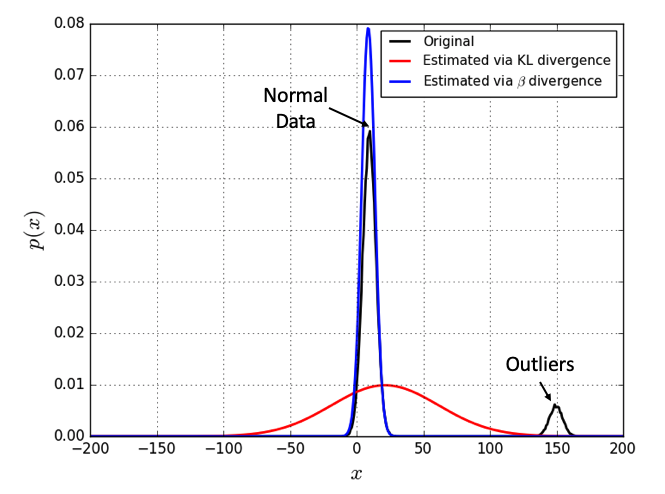
\includegraphics[scale=0.3]{./figures/simulations_compare_KL_with_beta.png}
	\caption{Illustration of robustness of $\beta$-divergence to outliers: optimizing KL-divergence for parameter estimation of Gaussian distribution attempts to also account for the presence of outliers, whereas optimizing $\beta$-divergence results in an estimate that is more robust to outliers.}	
	\label{fig:simulations_compare_KL_with_beta}
\end{figure}

\section{Variational Autoencoders}
\label{sec:variational_autoencoders}
In this section, we provide a review for VAEs. We adopt the notation in \citet{ghosh2019variational}. Let $\mathcal{X} = \left\{ \bx_i \right\}_{i=1}^N$ be high-dimensional i.i.d. samples drawn from the true data distribution $p_{\textrm{data}}(\bx)$ over a random variable $\bX$. Generative modeling aims to learn a mechanism from $\mathcal{X}$ to draw new samples such that $\bx_{\textrm{new}} \sim p_{\textrm{data}}$. VAEs provide a framework to achieve this goal by learning representation in low-dimensional latent space. The generative process of the VAE is defined as
\begin{equation}
\bz_{\textrm{new}} \sim p(\bZ) \quad \quad \quad \bx_{\textrm{new}} \sim p_{\theta}(\bX | \bZ = \bz_{\textrm{new}})
\end{equation}
where $p(\bZ)$ is a fixed prior distribution over latent space $\bZ$. A stochastic decoder
\begin{equation}
D_{\theta}(\bz) = \bx \sim p_{\theta}(\bx \mid \bz) = p(\bX | g_{\theta}(\bz))
\end{equation}
maps the latent variable to the input space via the \textit{likelihood} distribution $p_{\theta}$, where $g_{\theta}$ is a non-linear function, typically a neural network, parameterized by $\theta$. Consequently, a VAE estimates $p_{\textrm{data}}(\bx)$ as the infinite mixture model $p_{\theta}(\bx) = \int p_{\theta}(\bx \mid \bz) p(\bz) d\bz$. At the same time, the input space is mapped to the latent space via a stochastic encoder
\begin{equation}
E_{\phi}(\bx) = \bz \sim q_{\phi}(\bz \mid \bx) = q(\bZ \mid f_{\phi}(\bx))
\end{equation}
where $q_{\phi}(\bz \mid \bx)$ is the \textit{posterior} distribution given by another non-linear function $f_{\phi}$ parameterized by $\phi$.

Computing the marginal log-likelihood $\log p_{\theta}(\bx)$ is generally intractable. Therefore, it is common to follow a variational approach which focuses on maximizing the evidence lower bound (ELBO) for a sample  $\bx$:
\begin{equation}
\begin{split}
\log  &p_{\theta}(\bx) \geq  \textrm{ELBO}(\phi, \theta, \bx) \\
&= \mathbb{E}_{\bz \sim q_{\phi}(\bz \mid \bx)} \log p_{\theta}(\bx \mid \bz) - \mathbb{KL}(q_{\phi}(\bz \mid \bx) || p(\bz))
\end{split}
\label{eqn:elbo}
\end{equation}
Maximizing equation \ref{eqn:elbo} over data $\mathcal{X}$ with respect to parameters $\phi$ and $\theta$ corresponds to minimizing the loss
\begin{eqnarray}
\arg \min_{\phi, \theta} && \mathbb{E}_{\bx \sim p_{\textrm{data}}}  \mathcal{L}_{\textrm{ELBO}} \\
&=& \mathbb{E}_{\bx \sim p_{\textrm{data}}} \left[ \mathcal{L}_{\textrm{REC}} + \mathcal{L}_{\textrm{KL}} \right]
\end{eqnarray}
where $\mathcal{L}_{\textrm{REC}}$ and $\mathcal{L}_{\textrm{KL}}$ are defined for sample $\bx$ as follows:
\begin{eqnarray}
\mathcal{L}_{\textrm{REC}} &=& - \mathbb{E}_{\bz \sim q_{\phi}(\bz \mid \bx)} \log p_{\theta}(\bx \mid \bz) \\
\mathcal{L}_{\textrm{KL}} &=& \mathbb{KL}(q_{\phi}(\bz \mid \bx) || p(\bz)).
\label{eqn:L_rec_kl}
\end{eqnarray}
The reconstruction loss $\mathcal{L}_{\textrm{REC}}$ computes the quality of encoded samples $\bx$ through $D_{\theta} \left( E_{\phi}(\bx) \right)$. The KL-divergence term $\mathcal{L}_{\textrm{KL}}$ measures the similarity between $q_{\phi}(\bz \mid \bx)$ and the prior $p(\bz)$ for each $\bz$. This KL-divergence term is also called the regularizer term since it acts as a regularizer during training \cite{hoffman2016elbo}.
\section{Robust Variational Inference}
In this section, we show how the reconstruction term $\mathcal{L}_{\textrm{REC}}$ can be modified using a robust divergence in order to make it more robust to outliers for categorical data. Let empirical distribution of $\bX$ be
\begin{equation}
\hat{p}(\bX) = \frac{1}{N} \sum_{i=1}^N \delta(\bX, \bx_i)
\end{equation}
where $\delta$ is the Dirac delta function. The KL-divergence between this empirical distribution $\hat{p}(\bX)$ and $p_{\theta}(\bX | \bz)$ can be written as
\begin{equation}
\begin{split}
 & \mathbb{KL}\left(\hat{p}(\bX) || p_{\theta}(\bX | \bz)  \right) = \int \hat{p}(\bX) \log \frac{\hat{p}(\bX)}{p_{\theta}(\bX | \bz)} d \bX  \\
& \quad \quad = \textrm{const} - \int \hat{p}(\bX) \log p_{\theta} (\bX \mid \bz) d \bX  \\
& \quad \quad = \textrm{const} - \int \frac{1}{N} \sum_{i=1}^N \delta(\bX, \bx_i) \log p_{\theta}(\bX \mid \bz) d \bX \\
& \quad \quad = \textrm{const} - \frac{1}{N} \sum_{i=1}^N \log p_{\theta}(\bx_i \mid \bz)
\end{split}
\end{equation}
indicating that maximizing the log-likelihood of a sample $\bx_i$ is equivalent to minimizing KL-divergence between the empirical distribution and the generative distribution for one sample. Let the KL-divergence for a single sample $\bx_i$ be
\begin{equation}
\mathbb{KL}^i \triangleq -\frac{1}{N} \log p(\bx_i \mid \bz).
\end{equation}
Then, the reconstruction loss for a single sample can be written as
\begin{equation}
\mathcal{L}_{\textrm{REC}}^i = N \mathbb{E}_{\bz \sim q_{\phi}(\bz \mid \bx)} \left [ \mathbb{KL}^i \right ].
\end{equation}
The log-likelihood term $ \log p(\bx_i \mid \bz)$ in $\mathbb{KL}^i$ is sensitive to the outliers because the negative log-likelihood of low probability samples can be arbitrarily high. Rather than using KL-divergence, it is possible to choose a different divergence measure to quantify the similarity between $\hat{p}(\bX)$ and $p_{\theta} (\bX \mid \bz)$. We use $\beta$-divergence which is defined as
\begin{equation}
\begin{split}
\mathbb{D}_{\beta}(\hat{p}(\bX) ||  p_{\theta} (\bX & \mid \bz) = \\
 & \frac{1}{\beta} \int \hat{p}(\bX)^{\beta + 1} d \bX \\
&  - \frac{\beta + 1}{\beta} \int \hat{p}(\bX) p_{\theta}(\bX \mid \bz)^{\beta} d \bX \\
&  + \int p_{\theta}(\bX \mid \bz)^{\beta + 1} d \bX
\end{split}
\end{equation}
which converges to $\mathbb{KL}$ as $\beta \rightarrow 0$.  It can be shown that minimizing $\beta$-divergence is equivalent to minimizing $\beta$-cross-entropy \cite{eguchi2010entropy, futami2017variational} which is defined as
\begin{equation}
\begin{split}
\mathbb{H}_{\beta} & (\hat{p}(\bX) || p_{\theta}(\bX | \bz)) = \\
& - \frac{\beta + 1}{\beta} \int \hat{p}(\bX) \left(p_{\theta}(\bX | \bz)^{\beta}-1 \right) d \bX  \\ 
& \quad + \int p_{\theta}(\bX| \bz)^{\beta + 1} d \bX.
\end{split}
\label{eqn:beta_entropy}
\end{equation}

Since we are interested in applying VAE to a categorical data, we can assume  that the generative distribution is a categorical distribution with $K$ categories. Then, the first integral in equation \ref{eqn:beta_entropy} becomes:
\begin{equation}
\begin{split}
\int \hat{p}(\bX) &  p_{\theta}(\bX | \bz)^{\beta }d \bX = \\
& \frac{1}{N} \int \sum_{i=1}^N \delta(\bX, \bx_i) \left( p_{\theta}(\bX | \bz)^{\beta} - 1 \right) d \bX   \\
&= \frac{1}{N} \sum_{i=1}^N  \left( p_{\theta}(\bx_i | \bz)^{\beta} - 1 \right)
\end{split}
\end{equation}
The second integral can be written as:
\begin{equation}
\begin{split}
\int p_{\theta}(\bX | & \bz)^{\beta + 1} dX = \\
& \int \prod_{k=1}^K p_{\theta}( \bX == k \mid \bz)^{\beta + 1} \delta (\bX, k) d \bX  \\
&= \sum_{k=1}^K p_{\theta}(\bX == k \mid \bz)^{\beta + 1}
\end{split}
\end{equation}
Let's define $\beta$-cross-entropy for a single point as:
\begin{equation}
\begin{split}
\mathbb{H}_{\beta}^i &= - \frac{\beta + 1}{\beta} \frac{1}{N} \left( p_{\theta}(\bx_i \mid \bz)^{\beta} - 1 \right) \\
& \quad \quad + \frac{1}{N} \sum_{k=1}^K p_{\theta}(\bX == k \mid \bz)^{\beta + 1}.
\end{split}
\end{equation}
Then, the reconstruction loss for a single sample using $\beta$-divergence can be written as
\begin{equation}
\mathcal{L}_{\textrm{REC-} \beta}^i = N \mathbb{E}_{\bz \sim q_{\phi}(\bz \mid \bx)} \left [ \mathbb{H}_{\beta}^i \right ].
\label{eqn:L_rec_beta}
\end{equation}

\section{Wasserstein Autoencoders}
\label{sec:wasserstein_autoencoders}
Wasserstein autoencoders (WAE) \cite{tolstikhin2017wasserstein} allow us to use non-random decoders. This way, we do not need to perform Monte Carlo sampling for the reconstruction. The core idea behind WAE is to minimize Wasserstein distance between the $p_{\textrm{data}}(\bx)$ and $p_{\theta}(\bx)$ instead of maximizing the ELBO in equation \ref{eqn:elbo}. The authors of \citet{tolstikhin2017wasserstein}  show that minimizing Wasserstein distance between the $p_{\textrm{data}}(\bx)$ and $p_{\theta}(\bx)$  reduces to optimizing over random encoders which is basically the $\mathcal{L}_{\textrm{REC}}$ term in equation \ref{eqn:L_rec_kl}. However, they propose to replace the $\mathcal{L}_{\textrm{KL}}$ with \textit{maximum mean discrepancy} (MMD) or Jensen-Shannon divergence (as in \cite{goodfellow2014generative}) between $q_{\phi}(\bz \mid \bx)$ and $p(\bz)$. Using Jensen-Shannon entropy results in WAE-GAN and requires min-max optimization which can be challenging in practice. Therefore, we use MMD-based penalty in this work.

\subsection{Maximum Mean Discrepancy (MMD)}
\label{sec:mmd}
MMD \cite{gretton2012kernel} is a test statistic that is used to determine if two samples are from different distributions. It measures the largest difference in expectations over functions in the unit ball of a reproducing kernel Hilbert space (RKHS).
\begin{defn} \textbf{MMD:} \cite{tolstikhin2017wasserstein}
For a positive-definite reproducing kernel $k : \mathcal{Z} \times \mathcal{Z} \rightarrow \mathcal{R}$, the maximum mean discrepancy between $q_{\phi}(\bz \mid \bx)$ and $p(\bz)$ is defined as
\begin{equation}
\begin{split}
\mathbb{MMD}_k \left( q_{\phi}(\bz \mid \bx), p(\bz) \right) &= \left\| \int k(\bz,.) dq_{\phi}(\bz \mid \bx) \right. \\
& \left. - \int k(\bz, .) dp(\bz) \right\|_{\mathcal{H}_k}
\end{split}
\end{equation}
where $\mathcal{H}_k$ is the RKHS of real-valued functions mapping $\mathcal{Z}$ to $\mathcal{R}$ and the notation $k(\bz, .)$ indicates the kernel has one argument fixed at $\bz$ and the other argument is free.
\end{defn}
We refer \cite{tolstikhin2017wasserstein} for more detailed discussion on this. Fortunately, squared $\mathbb{MMD}$ has an unbiased U-statistic estimator which can be written as
\begin{equation}
\begin{split}
\mathbb{MMD}^2_u(\bz, \tilde{\bz}) &= \frac{1}{N(N-1)} \sum_{i=1}^N \sum_{j \neq i}^N k(\bz_i, \bz_j) \\
&+ \frac{1}{N(N-1)} \sum_{i=1}^N \sum_{j \neq i}^N k(\tilde{\bz}_i, \tilde{\bz}_j) \\
&- \frac{2}{N^2}  \sum_{i=1}^N   \sum_{j=1}^N  k(\bz_i, \tilde{\bz}_j)
\end{split}
\end{equation}
where $\tilde{\bz}_i$ are the samples from distribution $q_{\phi}(\bz \mid \bx)$ and $\bz_i$ are sampled from $p(\bz)$. Similar to \cite{tolstikhin2017wasserstein}, we use \textit{inverse multiquadratics} kernel $k(x, y) = C / (C + \|x - y \|^2_2)$ with $C = 2 d_z \sigma_z^2$ where $d_z$ is the dimension of $\bz$. Note that this $C$ is the expected squared distance between two multivariate Gaussian vectors drawn from $p(\bz)$ with standard deviation $\sigma_z$.
\section{Robust VAE with $\beta$ and MMD divergences (RVAE-MMD)}
\label{sec:proposed_approach}
In this section, we present our variational autoencoder using the concepts of $\beta$-cross-entropy and MMD discussed above. We derive the cost function we want to optimize as
\begin{equation}
\begin{split}
\phi, \theta = \arg \min_{\phi, \theta} \mathbb{E}_{\bx \sim p_{\textrm{data}}(\bx)} \left[ \mathcal{L}_{\textrm{REC-}\beta} + \mathcal{L}_{\textrm{MMD}} \right]
\end{split}
\end{equation}
where $\mathcal{L}_{\textrm{REC-}\beta}$ represents the loss term per sample introduced in equation \ref{eqn:L_rec_beta} and $ \mathcal{L}_{\textrm{MMD}}$ is the regularization term that uses MMD as a dissimilarity measure in latent dimension. Using the empirical estimates of expectation over $p_{\textrm{data}}(\bx)$,  we can write:
\begin{equation}
\begin{split}
\phi, \theta = \arg \min_{\phi, \theta} & \left[ - \frac{\beta+1}{N \beta} \sum_{i=1}^N \left( p_{\theta}(\bx_i \mid \tilde{\bz}_i)^{\beta} - 1 \right)  \right. \\ 
& +  \sum_{k=1}^K p_{\theta}(\bX == k \mid \tilde{z}_i)^{\beta+1} \\
& + \frac{1}{N(N-1)} \sum_{i=1}^N \sum_{j \neq i}^N k(\bz_i, \bz_j) \\
&+ \frac{1}{N(N-1)} \sum_{i=1}^N \sum_{j \neq i}^N k(\tilde{\bz}_i, \tilde{\bz}_j) \\
& - \left. \frac{1}{N^2}  \sum_{i=1}^N   \sum_{j=1}^N  k(\bz_i, \tilde{\bz}_j) \right]
\end{split}
\end{equation}
where each $\bz_i$ is sampled from $p(\bz)$ and $\tilde{\bz}_i$ is the output of the encoder given $\bx_i$. The details for training RVAE-MMD are given in Algorithm \ref{alg:rvae_mmd}. Note that we use non-random decoder $p_{\theta}(\bx \mid \bz)$ which means that we deterministically map latent variable $\bz$ to the original dimensional variables $\bx$. Also, we use inverse multiquadratics kernel defined in Section \ref{sec:mmd}.

\begin{algorithm}[!h]
   \caption{Training RVAE-MMD}
   
   \textbf{Input:} 
   
	\hspace{\parindent} Initialize the parameters of the encoder $q_{\phi}(\bz \mid \bx)$ and the decoder $p_{\theta}(\bx \mid \bz)$.
	
	\hspace{\parindent} Define the kernel $k$ to compute $\mathbb{MMD}$.
	
	\hspace{\parindent} Robust divergence coefficient $\beta \geq 0$.

   \textbf{Output:} 
	\hspace{\parindent} $\phi$, $\theta$

\begin{algorithmic}[1]
   \WHILE{$\phi$ and $\theta$ not converged}
   \STATE Sample $\{\bx_1, \cdots, \bx_N \}$ from the training set
   \STATE Sample $\{\bz_1, \cdots, \bz_N \}$ from the prior $p(\bz)$
   \STATE Sample $\{\tilde{\bz}_1, \cdots, \tilde{\bz}_N \}$ from $q_{\phi}(\bz \mid \bx_i)$
   \STATE Compute $\beta$-divergence term: \\\quad$\mathcal{L}_{\textrm{REC-}\beta} = - \frac{\beta+1}{N \beta} \sum_{i=1}^N \left( p_{\theta}(\bx_i \mid \tilde{\bz}_i)^{\beta} - 1 \right)$ \\  \quad \quad  \quad \quad \quad $+ \sum_{k=1}^K p_{\theta}(\bX == k \mid \tilde{z}_i)^{\beta+1}$
   \STATE Compute MMD term: \\\quad $\mathcal{L}_{\textrm{MMD}} = \frac{1}{N(N-1)} \sum_{i=1}^N \sum_{j \neq i}^N k(\bz_i, \bz_j)$\\  \quad \quad  \quad \quad \quad $+\frac{1}{N(N-1)} \sum_{i=1}^N \sum_{j \neq i}^N k(\tilde{\bz}_i, \tilde{\bz}_j)$ \\  \quad \quad  \quad \quad \quad  $- \frac{2}{N^2}  \sum_{i=1}^N   \sum_{j=1}^N  k(\bz_i, \tilde{\bz}_j)$
   \STATE Update $\phi$ and $\theta$ by descending the total loss \\\quad $\mathcal{L}_{\textrm{TOT}} = \mathcal{L}_{\textrm{REC-}\beta} + \mathcal{L}_{\textrm{MMD}} $
   \ENDWHILE
   \STATE Return $\phi$, $\theta$
\end{algorithmic}
\label{alg:rvae_mmd}
\end{algorithm}

\section{AWS CloudTrail}
In this section, we review AWS CloudTrail \cite{aws_cloudtrail} service since our motivating application for the RVAE-MMD is to detect abnormal activities in AWS accounts. AWS CloudTrail enables logging and monitoring AWS account activities taken through AWS Management Console, AWS SDKs, command line tools, and other AWS services. Hence, it provides a rich source of information that can be used for compliance, operational auditing, and risk auditing of AWS accounts. As a result, CloudTrail events can be used to detect unusual activities carried out by attackers using stolen AWS credentials. For example, any unusual activity in highly sensitive operations such as CreateSecurityGroup or AuthorizeSecurityGroupIngress could be suspicious. Another example is a user logging on to AWS console from the other side of the world instead of a neighboring network. Detecting such events warrant alerting the AWS user.

Amazon GuardDuty -- AWS' threat detection service \cite{aws_guardduty} -- monitors CloudTrail events along with other sources such as AWS VPC Flow Logs and DNS Logs to identify potential threats. However, there is not a systematic way of using CloudTrail events despite the huge potential. The current service is still rule-based which requires manual definitions of rules. Furthermore, the rule based decisions are easily plagued by large false positive rates because users regularly generate new but legitimate activities.

In this work, our goal is to automate this process by utilizing machine learning algorithms. One of the challenges with working on CloudTrail data is its high-cardinality of categorical features such as IP address, userID, eventName, etc. Therefore, we cannot directly apply previously proposed techniques designed for numerical or image datasets. 

\subsection{Previous Work on CloudTrail Events}
At AMLC 2019, \citet{coskun2019detecting} proposed an end-to-end unsupervised machine learning approach for detecting anomalous CloudTrail events. To mitigate the high-dimensionality problem, they proposed to learn embeddings (vector representations) as part of model training that captures semantic similarities between features. However, even after embeddings, the dimensionality of the event space is still large and sparse. To handle this challenge further, they suggested to consider each event in its own context which usually constitutes a much smaller space. In addition to reducing the dimensionality, this approach leads to learning abnormalities on user level instead of global level. The advantage of this approach is that a globally rare event can be normal for some users and, on the contrary, a globally normal event can be an anomaly for some other users.

Along with this conditional modeling strategy and embeddings, \citet{coskun2019detecting}  adopted a WAE model and demonstrated improved performance compared to rule-based and VAE-based approaches. We have been notified by the authors that the WAE model is scheduled to be deployed within AWS-GuardDuty.  In our experimental results on CloudTrail events, we use their approach as baseline.

\section{Experiments on Cloud Trail Events Data}
 \begin{figure*}[h!]
	\centering
	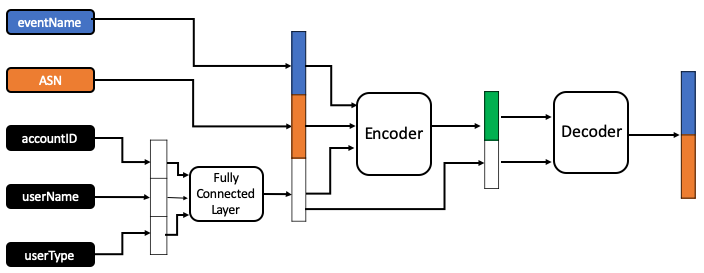
\includegraphics[scale=.5]{./figures/architecture.png}
	\caption{Neural network architecture based on conditional VAE. Each event is considered in its own context and the context of each event is defined as (\texttt{accountID}, \texttt{userName}, \texttt{userType}).}
	\label{fig:architecture}
\end{figure*}
\subsection{Modeling Cloud Trail Events}
CloudTrail events consist of various different features.  Similar to \cite{coskun2019detecting}, we use five specific features which are present in all CloudTrail events. 
We define each CloudTrail event as the following five-tuple: 
\begin{center}
\small
(\texttt{accountId}, \texttt{userName}, \texttt{userType}, \texttt{eventName}, \texttt{ASN})
\end{center}
where ASN stands for Autonomous System Number.  ASN can be considered as the identifier of the internet service provider which owns the IP address. The reason why we use ASN instead of IP address is two-fold: (i) unique number of ASNs (around 65K) is less than the unique number of IP addresses (can be as large as $2^{32}$) which simplifies vector representations, and (ii) IP address is volatile and may change frequently under the same ASN.

Following the conditional modeling, each event is considered in its own context. The context of each event is defined by \texttt{accountID}, \texttt{userName} and \texttt{userType}. Hence, instead of  modeling the joint distribution 
\begin{equation}
p(\textrm{accountId}, \textrm{userName}, \textrm{userType}, \textrm{eventName}, \textrm{ASN}), \nonumber
\end{equation}
 we model the conditional distribution 
 \begin{equation}
 p(\textrm{eventName}, \textrm{ASN} \mid \textrm{accountId}, \textrm{userName}, \textrm{userType}) \nonumber
\end{equation} 
  which is easier to estimate since the conditional probability space is much smaller. Modeling  this conditional probability allows us to adopt conditional VAE approach \cite{sohn2015learning}.

Finally, as previously done in~\cite{coskun2019detecting}, we compare the proposed model with some of the existing GuardDuty rules which are used in production to generate findings,
and report the results from best performing rules, namely “API Called From Unseen Internet Service Provider (ISP)” and “API Called From Unseen ASN".

\subsection{Network Architecture}
We illustrate the neural network architecture in Figure \ref{fig:architecture}. The model consists of fully-connected layer that maps the embedding of each context to a joint representation. The output of this fully-connected layer is concatenated to the embeddings of event information. The encoder encodes the concatenated embeddings into a latent space. In order to make the model conditional, we feed the output of the encoder along with the context information to the decoder. Finally, we reconstruct embeddings of  \texttt{eventName} and \texttt{ASN} from the decoder. Since the features are categorical, we use SoftMax layer in the output of decoder to reconstruct the events.
We use deterministic encoder and decoder both for  the WAE and our RVAE-MMD. Finally, we use reconstruction probability as anomaly score.
% \small{
\begin{table*}[h!]
	\centering
	% \begin{tabular}{p{.8cm}p{.8cm}p{1.3cm}p{1.3cm}p{.4cm}p{1cm}}
	\begin{tabular}{lp{.8cm}p{1.3cm}p{1.3cm}p{1.3cm}p{1.3cm}}
			\toprule
		\textbf{Model}  &$\beta$ &\textbf{Precision} (\%) & \textbf{Recall} (\%)  &\textbf{F1} (\%) & \textbf{LossRatio} \\
		\midrule
		WAE & N/A & XXX & \textbf{XXX} & XXX & XXX \\

		\bottomrule
	\end{tabular}
	\caption{Performance metrics on test data for different models trained on two-accounts data. The loss ratio is computed on $90$ normal and $10$ attack samples from the validation dataset.}
\label{tab:two_accounts}
\end{table*}
% }

\subsection{Computational and Implementation Details:} 

We use Python 3.6 for implementation \cite{oliphant2007python} using open-source libraries MXNet \cite{mxnet2018flexible}, scikit-learn \cite{pedregosa2011scikit},  and NumPy \cite{walt2011numpy}. Experiments are run using Amazon EC2 P3 instances. We use Adam \cite{kingma2014adam} as an optimizer with learning rate $1e-3$ and bias correction parameters $0.5$ and $0.999$ for gradients and squared gradients, respectively. We vary the $\beta$ parameter from $1 e-5$ to $0.1$ in logarithmic scale.

\subsection{Model Selection}
We perform model selection on validation dataset consisting of a few attack and normal samples. More specifically, we compute the cross-entropy loss from both attack and the normal samples and then compute the ratio of these losses:
\begin{equation}
\mbox{LossRatio} = \frac{\frac{1}{{N}} \sum_{i=1}^N - \log p_{\theta}(\bx_i \mid f_{\phi}(\bx_i)) }{ \frac{1}{{A}}   \sum_{i=1}^A- \log p_{\theta}(\bx_i \mid f_{\phi}(\bx_i)) }
\end{equation}
where $N$ is the total number of normal samples and $A$ is the total number of attack samples in the validation dataset. For a robust outlier detection model, we expect the numerator to be as small as possible and the denominator as large as possible. Hence, we can conclude that smaller LossRatio indicates more robust models. Therefore, in the following experiments, we compute this LossRatio on validation dataset and select the best epoch number and $\beta$ parameter for RVAE-MMD based on the smallest LossRatio.






\section{Conclusion}
We proposed a robust VAE using $\beta$ and MMD divergences to guarantee robustness to outliers in training data. Our experimental results on CloudTrail events show that our approach can yield more accurate results than the WAE model, which is scheduled for production. The improvement with our approach is even more significant when the training data is contaminated even with small amount of outliers. Encouraged by these results, we plan to replace the production WAE model with our proposed model in the future once we incorporate tuning $\beta$ parameter process into our production pipelines. Although we applied our approach to CloudTrail events, our approach can be applied in other Amazon services for cyber-security, fraud, and abuse prevention on Amazon AWS and retail platforms.

Our approach has potentially broader impact in general machine learning field. As future work, we plan to compare our approach with existing unsupervised learning approaches specifically for categorical data on benchmark datasets for external publications. Furthermore, we plan to extend this approach to semi-supervised problems and supervised problems with noisy labels.

\bibliography{mybib}
\bibliographystyle{icml2020}
%
%\section{Appendix}
\end{document}


% This document was modified from the file originally made available by
% Pat Langley and Andrea Danyluk for ICML-2K. This version was created
% by Iain Murray in 2018, and modified by Alexandre Bouchard in
% 2019 and 2020. Previous contributors include Dan Roy, Lise Getoor and Tobias
% Scheffer, which was slightly modified from the 2010 version by
% Thorsten Joachims & Johannes Fuernkranz, slightly modified from the
% 2009 version by Kiri Wagstaff and Sam Roweis's 2008 version, which is
% slightly modified from Prasad Tadepalli's 2007 version which is a
% lightly changed version of the previous year's version by Andrew
% Moore, which was in turn edited from those of Kristian Kersting and
% Codrina Lauth. Alex Smola contributed to the algorithmic style files.




%%%%OLD TABLES% \begin{table}[htbp]
% %	\scriptsize
% 	\centering
% 	\begin{tabular}{p{1.2cm}p{1.6cm}p{1.6cm}p{1.6cm}} \\ \toprule
% 	\textbf{Model} & \textbf{No added outliers} & \textbf{0.0025 \% outliers} & \textbf{0.025 \%  outliers} \\ \midrule
% 	RWAE & 0.9688 & 0.941 & 0.9392 \\
% 	WAE & 0.9507 & 0.937 & 0.8977 \\ 
% 	\bottomrule
% 	\end{tabular}
% 	\caption{Precision@k=48 for the model with 500 accounts}
% 	\label{table:preck500}
% 	\end{table}

% \begin{table}[htbp]
% %	\scriptsize
% 	\centering
% 	\begin{tabular}{p{1.2cm}p{1.6cm}p{1.6cm}p{1.6cm}} \\ \toprule
% 	\textbf{Model} & \textbf{No added outliers} & \textbf{0.0025 \% outliers} & \textbf{0.025 \%  outliers} \\ \midrule
% 	RWAE & 0.982 & 0.9457 & 0.9402 \\
% 	WAE & 0.979 & 0.9423 & 0.9073 \\
% 	\bottomrule
% 	\end{tabular}
% 	\caption{PRAUC for the model with 500 accounts}
% 	\label{table:prauc500}
% 	\end{table}

% \begin{table}[htbp]
% %	\scriptsize
% 	\centering
% 	\begin{tabular}{lllll} \\ \toprule
% 	\textbf{Model} & \textbf{Precision} & \textbf{Recall} & \textbf{F1} & \textbf{PRAUC} \\ \midrule
% 	RWAE & 0.9903 & 0.9968 & 0.9936 & 0.9990 \\
% 	WAE & 0.9681 & 0.9965 & 0.9821 & 0.9984 \\ 
% 	\bottomrule
% 	\end{tabular}
% 	\caption{Alpha Dataset: Training Window 1}
% 	\label{table:alphawindow1}
% 	\end{table}

% \begin{table}[htbp]
% %	\scriptsize
% 	\centering
% 	\begin{tabular}{lllll} \\ \toprule
% 	\textbf{Model} & \textbf{Precision} & \textbf{Recall} & \textbf{F1} & \textbf{PRAUC} \\ \midrule
% 	RWAE & 0.9764 & 0.5404 & 0.6957 & 0.8029 \\
% 	WAE & 0.9650 & 0.4544 & 0.6179 & 0.7454 \\ 
% 	\bottomrule
% 	\end{tabular}
% 	\caption{Alpha Dataset: Training Window 2}
% 	\label{table:alphawindow2}
% 	\end{table}
